\documentclass[11pt,a4paper]{report}
\usepackage[utf8]{inputenc}
\usepackage{hyperref}
\usepackage{graphicx}
\usepackage{datetime}
\usepackage{color}
\usepackage{url}

\newcommand{\hi}[1]{{\color{red}\em #1\/}\\}
\newcommand{\todo}[1]{\footnote{{\color{red} {\bf TODO:} #1}}}
\newcommand{\ask}[1]{\footnote{{\color{red} {\bf QUESTION:} #1}}}

\begin{document}
\title{Product Report \\
  ``Treacherous Talks''}
\date{\today\ @ \currenttime}
\author{Dilshod Aliev, Jan Daniel Bothma, Stephan Brandauer,\\
 Andre Hilsendeger, Rahim Kadkhodamohammadi, Xinze Lin,\\
Tiina Loukusa, Erik Timan, Sukumar Yethadka}
\maketitle
\tableofcontents

\abstract{
Treacherous Talks is an implementation of a board game (``Diplomacy'') as a web
service.

We developed the service completely in Erlang while spending lots of time on
optimizing performance and scalability. The project was mostly self organized
by an international team of 9 students and developed using Scrum.
}

\chapter{Introduction}
Diplomacy is a board game, invented in the 1950s where the goal is to try to 
conquer Europe just before WW I. You come close to this goal by talking to the
other players --- by diplomacy --- and making them your allies. And you achieve
it by attack them when they do not expect it.

The game is and was commonly played over distance --- starting with playing by 
mail, then email and nowadays over pretty web pages with full-blown map
visualization.

The requirements we were faced with asked for implementation of Diplomacy as a
web service while providing several interfaces to this service. Scalability and
Failure Tolerance were of high priority. \\
Even though a board game is a fun thing to implement, we do think that the most
interesting part of our project is the scalability- and fault tolerance-
engineering.

\chapter{Preliminaries}
\hi{Describe important concepts, acronyms, tools you used in the process, target platforms, etc.}
\ask{regarding Releases, Applications: can we assume erlang-knowledge?}
\section{Releases}
\section{Applications}
\section{Scalability vs. Performance}

\chapter{System Description}
%\hi{System architecture, how it works.
%This is the core of your report, and is therefore most likely the largest section.}

\section{Requirements}

\subsection{Three Interfaces}
The requirement stated that we have to provide three interfaces that expose
the same functionality to the user (the operator is forced to use the
web~interface). Those interfaces are:\\
\begin{enumerate}
\item {\bf Web interface} ---
  the game should be accessible via a modern webbrowser {\em and\/} it should
  use websockets to communicate with the browser.
\item {\bf XMPP interface} --- 
  the game should be accessible via a chat client using text based orders.
\item {\bf SMTP interface} ---
  the game should be accessible via sending of emails using text based orders.
\end{enumerate}

\subsection{Scalability}
The system should be scalable. Scalability in this context refers to horizontal scaling where the system should be able to handle more load by simply adding more nodes. No further explanations were provided regarding this feature, but since we saw it as a challenge we invested a lot of work into it.

\subsection{Fail-Safety}
The system should be highly available. We interpreted this by assuming that we
should handle hardware failure of physical machines. As with scalability, we
might have been able to get away with less work but this feature as well was
too interesting too resist focusing on it.

\subsection{Websockets}
Websockets are a tcp-like connection between a browser and a webserver.
They can be used to send javascript that updates only parts of the client page
instead of reloading a page and are a great tool to shift computing to the 
client side.

The websockets feature was mostly an issue because of the tool support (or lack
thereof) we were faced with. More is explained in Sec.~\ref{sec:frontends}.
Otherwise, websockets are an amazing technology and will have a great impact on
web development in the future.

\subsection{AI}
Writing a simple AI was a requirement which interested us as well. However, we
were stuck in a tradeoff because time was limited: fail-safety+scalability
vs.\ AI players. In combination with our customer, we agreed on focusing on the
performance characteristics and leaving the AI players for future work.

\section{Architecture}
\subsection{Overview}
\todo{How modules communicate with each other}
% http://redmine.pcs/projects/dip/wiki/Communication
\todo{Supervision tree}
% http://redmine.pcs/projects/dip/wiki/Supervision_tree
\todo{How we deal with concurrency and conflicts}
% http://redmine.pcs/projects/dip/wiki/Concurrency_handling

\begin{figure}[h]
 \centering
 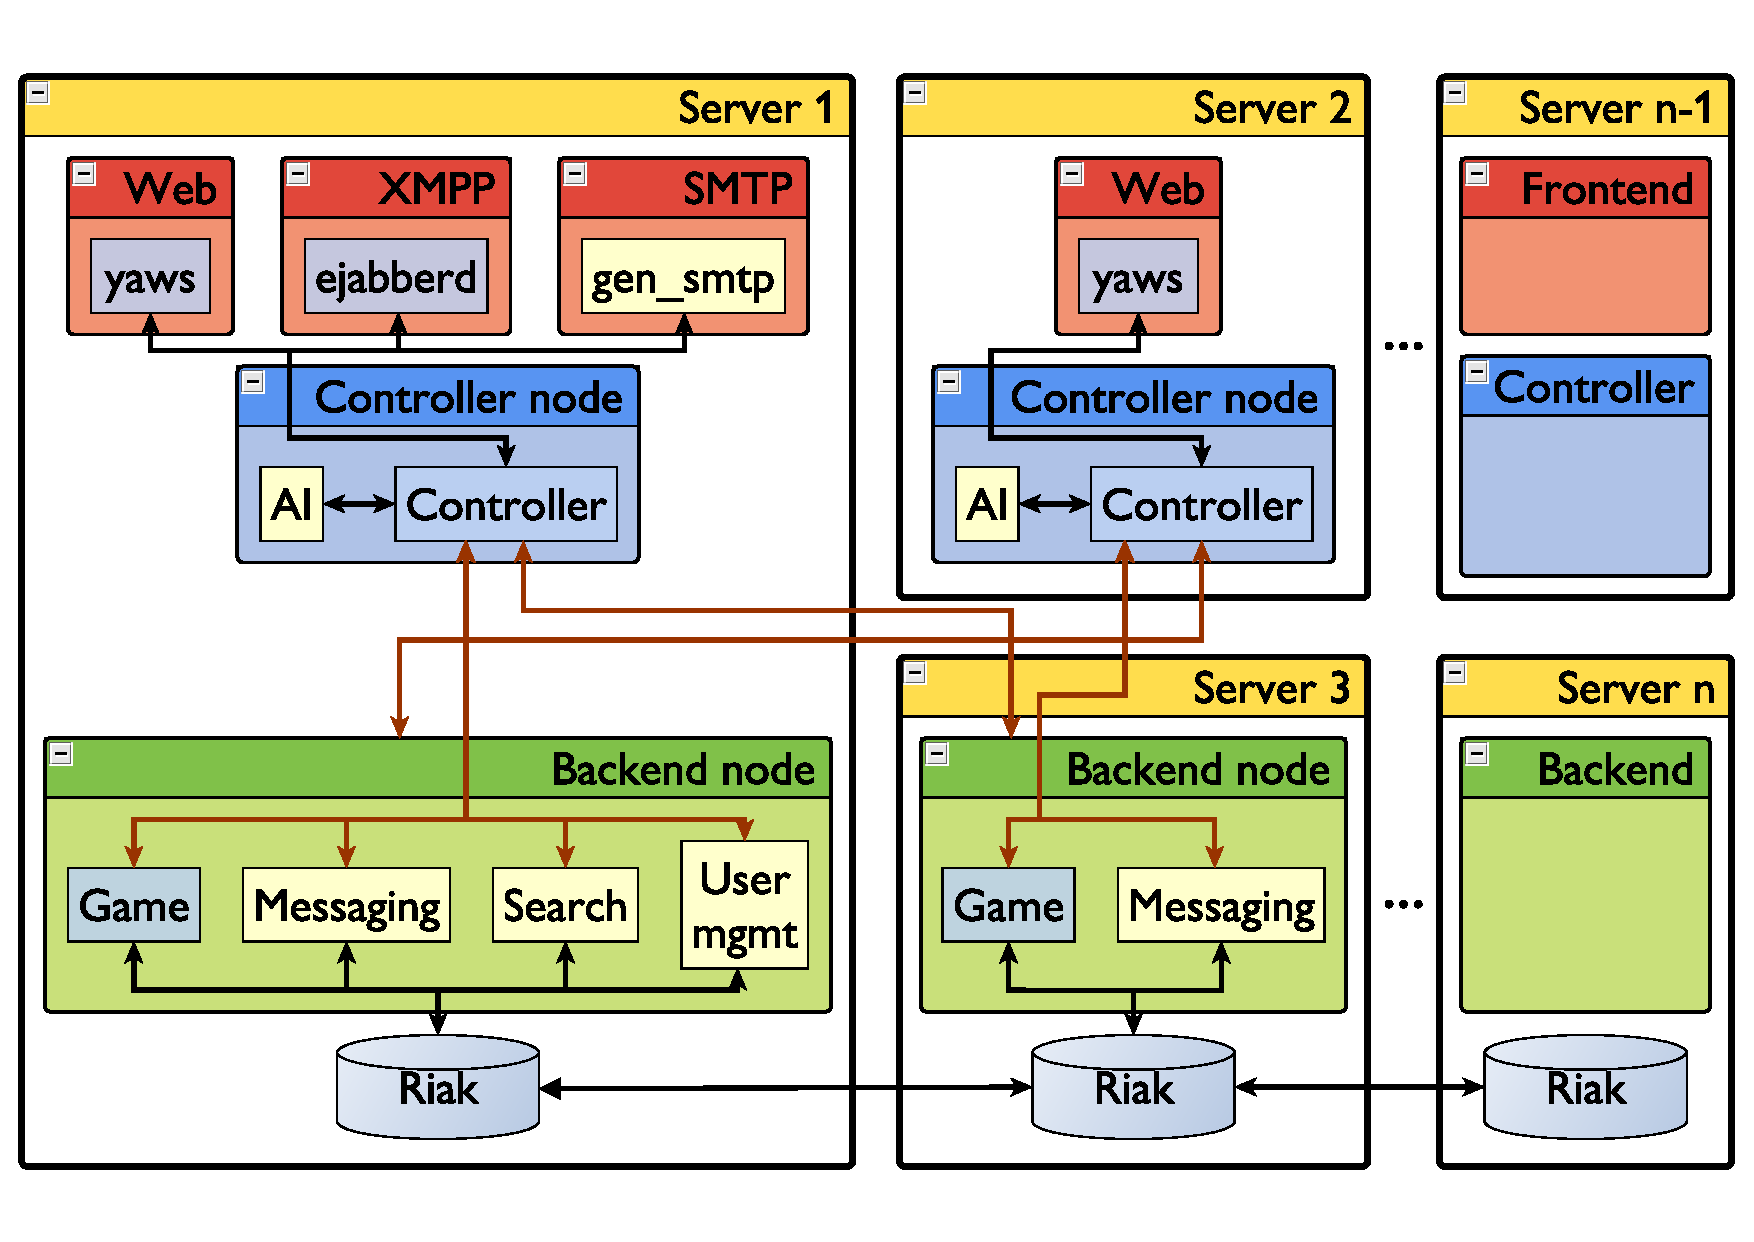
\includegraphics[width=13cm]{./graphics/arch.pdf}
 \caption{a possible cluster}
 \label{fig:arch}
\end{figure}

Our Architecture is divided in three main blocks, the {\em frontends}, the 
{\em controller}, and the {\em backends}. In Fig.~\ref{fig:arch} a running
cluster as it could be configured is shown. {\em Machine 1} shows a full
configuration as it includes all three frontends, a backend and riak. The
operator, however, is free to choose to only run a specific selection of these
and can combine them freely.

The responsibilities are not surprising: the frontends receive user input and
transform the input into messages which are sent to the controller.
The controller filters out illegal messages according to the session database
and the user privileges before handing them off to the backends --- which will
respond with an answer.
\subsubsection{Modularity --- and its Relation to Scalability}
One thing that is not immediately visible in our architecture is the fact that
the individual modules are very independent of each other. Even though the
architecture graphic shows a complete example of a running sample, we can choose
to run some modules alone. \\
If we would, for example, find out that our system is slow because the
web~frontend is the bottleneck, we could add more servers to the cluster that
run only a web~frontend (see Fig.~\ref{fig:arch}, ``Server n-1'').
We can do the same with each frontend types, with backends and with riak nodes.
Our architecture, therefore, inherently supports scaling out very well.
Since the frontends are not relying on each other at all (they are completely
parallel), we did not spend resources on load testing them since we needed that
time to benchmark and load test our backends and riak nodes.
\subsection{Frontends}
\label{sec:frontends}
The frontends spoke almost the same language to the user, which made the
implementation of front-end logic very generic.

\subsubsection{Web}
The web frontend is running yaws as a web server, after deciding to use nitrogen
as a web framework, we had to drop nitrogen because of the websockets
requirement. Yaws is configured as a ``/" application module (appmod) so that we can have a single entry point for handling all the requests. Server side includes (ssi) are also used to load static content via ajax.

The web frontend relies heavily on javascript since it contains a good part of the application logic handling user interactions, requests, responses and game functionalities. We also use the toolkit Bootstrap\ref{bootstrap} for the user interface which allows us to quickly develop clean pages.

\todo{People involved: explain the trouble with websockets}

\subsubsection{XMPP}
Using ejabberd as XMPP server was an obvious choice since ejabberd is widely
regarded as the standard solution for XMPP servers and ejabberd is implemented
in Erlang which led us to hope that it would play well with our code. \todo{People involved: tell a story}
\subsubsection{SMTP}
\todo{Lin: explain}

\subsection{Controller}
\subsubsection{Session Management}
\todo{People involved: explain}

\subsubsection{Access Control}
What users can perform what actions on the system is defined by a set of identities known as roles. The system has four roles.

\begin{itemize}
\item User - registered member of the system who can create and play games
\item Blacklisted user - a user who has been removed from the system
\item Moderator - a user with enhanced privileges to moderate games and help other users
\item Operator - an administrator who has complete control over the system

\end{itemize}

\subsection{Backend}
\subsubsection{Game Managing}
Managing games was split up in two main tasks: {\em game timing\/} and
{\em order-processing}. \\
Game timing was implemented as a {\tt gen\_fsm} that changes states when a game
phase needs to stop, eg.\ when the deadline for handing in orders is over.\\
Before a phase is started, the rules processing is done by a module we call
the ``rule engine'': the orders which were sent by the users before the deadline
are read from the database and passed, along with the current game map to the
rule engine.
\subsubsection{Messaging}
Since communication is very important in the game --- some even say, that the
game is mostly about communication --- the messaging module was a very central
feature for us. We support two types of messages: {\em in-game\/} and
{\em off-game\/}-messages.\\
Messages in game never involve the user name for
tactical reasons: if someone remembers my nickname, he has an easier time to
anticipate my moves since he will most likely remember my actions in last games.
Or, worse: he might still hold a grudge against me. This is why you never
communicate with players in-game by using their nickname, but by using their
country.

Off-game messages on the other hand are sent to a nickname and the recipient
will see the sender's nickname. The basic usecase for the off-game messaging is
giving users the chance to set up games for their friends and tell them about
it.
\subsubsection{Search}
Our search module provides the functionality to search, for instance, for games,
based on their properties (like all game parameters). For the implementation of
search, we relied on the riak extension {\tt riak\_search}. 

Riak search is a search engine that is tightly coupled with the Riak datastore. We add a precommit hook to the properties of the bucket whose data is to be searched along with search schema which specifies how the object is to be indexed. Whenever a new object is added or an old one updated, the object is indexed (tokenization with standard Lucene analyzers) and saved. It provides a rich query language consisting of term searches, field searches, boolean operators and wildcards to fetch matching objects ordered by relevance.

\todo{Andre: explain performance problems}
\subsubsection{User Management}
The user management module was one of the first modules we implemented in the
backend; its purpose is to create, update, read, delete users in or from the
database. The implementation is quite short and should contain few surprises.

\subsection{Riak}
The choice of riak as database was a carefule one: we evaluated riak, couchDB
and mnesia but riak was our favourite in the end --- it's scalability features
are very simple to use and it's potential for scalability is what we needed.
For managing of sessions, we had to resort to using mnesia for one class of
data:\todo{people involved: explain}. \\
Riak proved to be a good choice for us since its performance parameters (called
``CAP controls'' in riak-lingo) are very easy to tune and it is quite well
documented how riak behaves under load. The scalability problems we had
came from using the search module too much and in places where we shouldn't
have.
\subsubsection{eleveldb}
Another problem was riak's storage backend. Riak has the feature to switch the
storage backend --- the way, key/value pairs are stored on a node.
We initially used {\tt eleveldb} because it supported secondary indices, a
feature we wanted to use. {\tt eleveldb} however showed degrading performance
in our context: the throughput of database operations was decreasing linearly
over time, down to zero. We could not find out, what the problem here was, so
we had to switch the storage backend to {\tt bitcask}, riak's standard storage
backend. Bitcask does not support secondary indices, and because of that it was
necessary to use {\tt riak\_search} more --- which led to scalability
issues\ldots

\chapter{Treacherous Talks}
\hi{Describe the product from a user perspective, what you can do / what it looks like.}
\section{The Three Interfaces}
\subsection{HTTP}
The user goes to the landing page, there he finds a link to register which will
display a simple form for him to fill out. After the user is registered, he is
able to log in using the login textfields on the landing page.

After logging in, the user is shown an overview page (see Fig.~\ref{fig:overview})
 where he is able to search, look at the games he is playing in (if any) and chat
with other users in-game or off-game.

\begin{figure}[h]
 \centering
 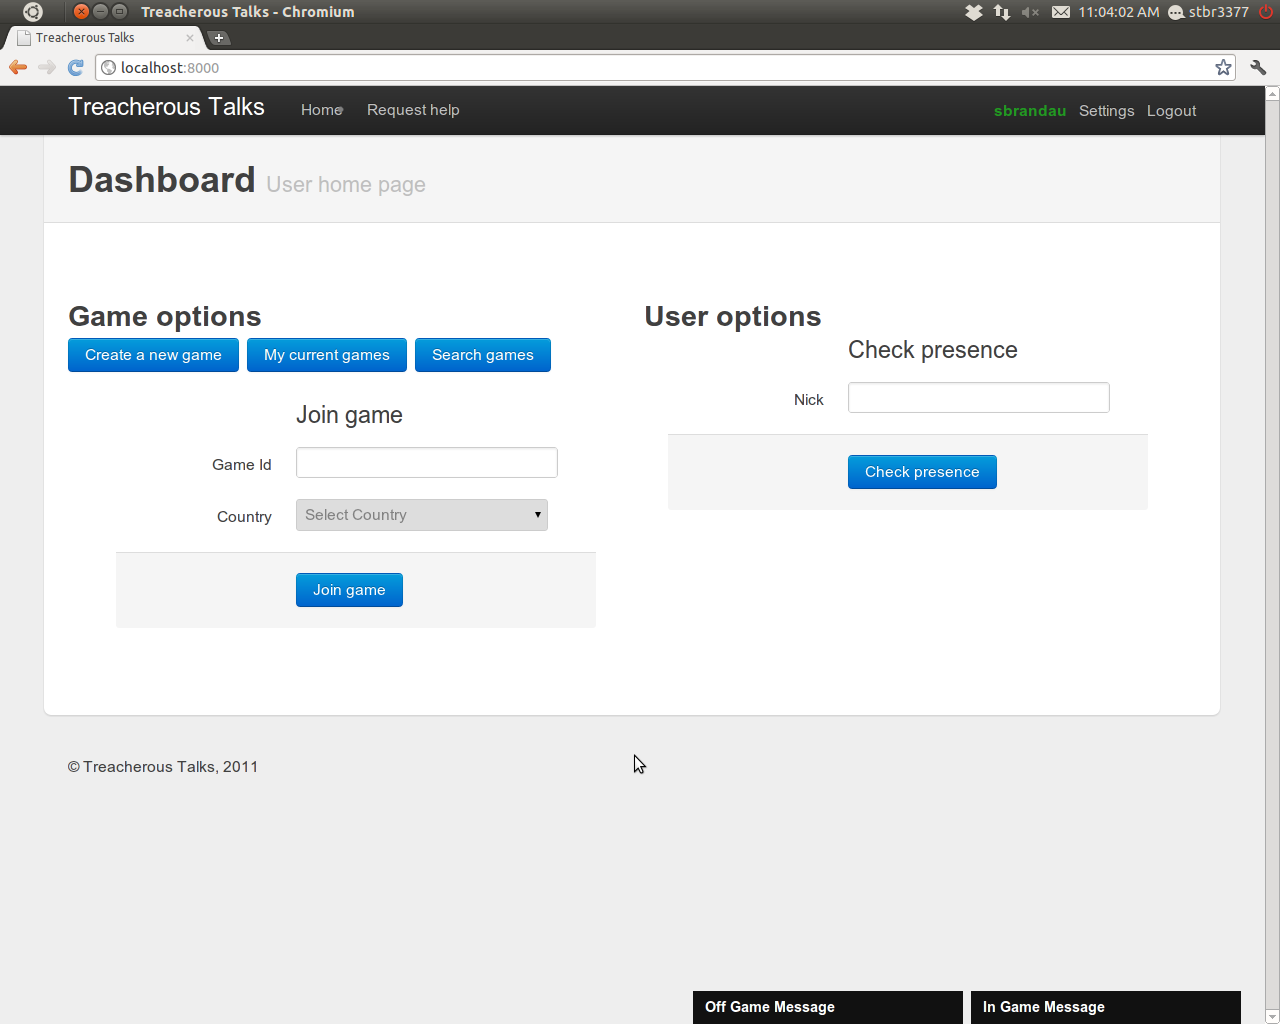
\includegraphics[width=\textwidth]{./graphics/overviewpage.png}
 \caption{the overview page}
 \label{fig:overview}
\end{figure}

The web frontend has several key advantages over the two purely text based
frontends:\\
\begin{itemize}
\item the user does not need to remember his session id
\item the user sees a graphical map (generated using a HTML5 canvas!),
  see Fig.~\ref{fig:map}
\item it is easier to enter move orders because possible orders are represented
  as drop-down lists, see Fig.~\ref{fig:orders}
\end{itemize}

\begin{figure}[h]
 \centering
 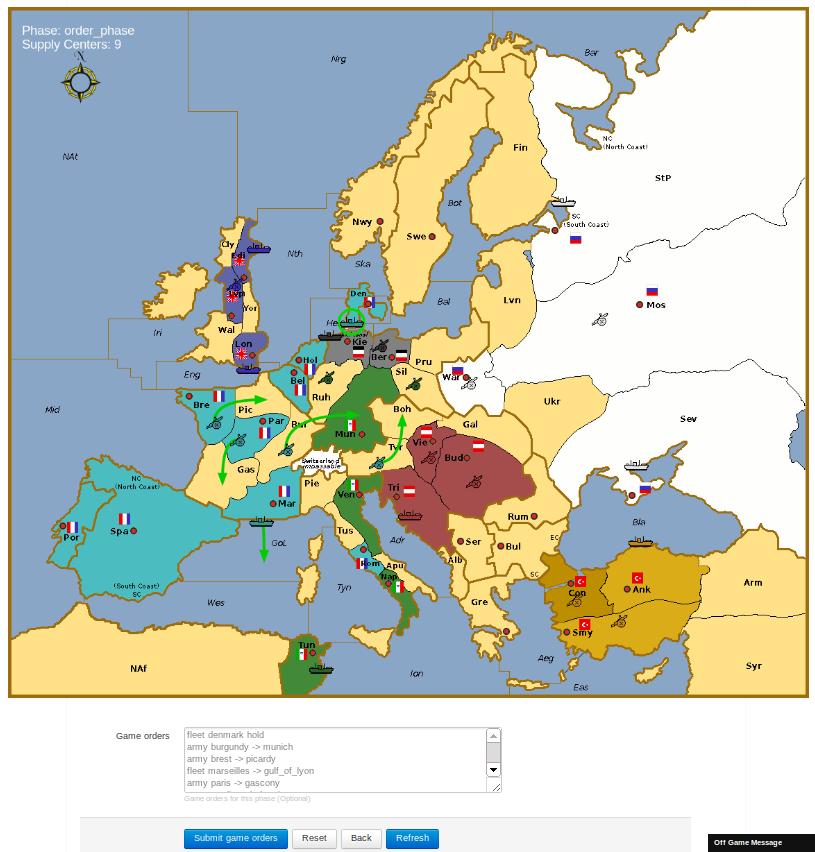
\includegraphics[width=10cm]{./graphics/graphicalmap.png}
 \caption{the graphical map}
 \label{fig:map}
\end{figure}

\begin{figure}[h]
 \centering
 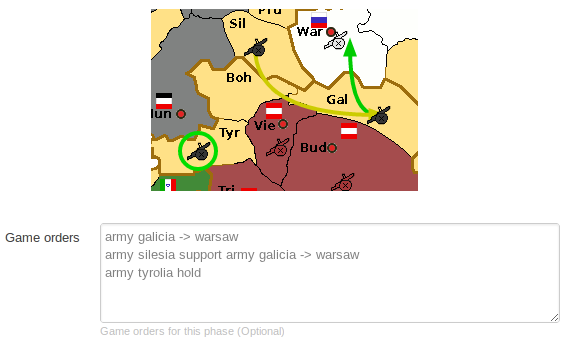
\includegraphics[width=10cm]{./graphics/orderssmall.png}
 \caption{the orders drop-down lists}
 \label{fig:orders}
\end{figure}


\subsection{XMPP}
\todo{Rahim: explain}
\subsection{SMTP}
\todo{Lin: explain}
\section{Messages}
In the web frontend, the user is shown two chat boxes: one for off-game chat
and one for ingame-chat. The user manually has to enter the recipient (in
in-game chat the recipient-country and the game ID). If the recipient is not
online when a message is sent, it will be stored and delivered by the message
application after the recipient logs in the next time. \\
\todo{People involved: explain text based message sending}

\section{Playing}
The web frontend generates drop down lists to make it easier for the user to
enter move orders. \todo{screenshot of drop down lists after feature freeze}
\todo{People involved: explain text based move orders}.

\chapter{Evaluation and Testing}
%\hi{Describe what experiments you have done to test your product.}
\section{Overview}
We approached testing very seriously from the start and are confident that this
was one of the best decisions we made throughout the project. Unit tests are too
low level to be covered here but they are of course there. We used EUnit for
most of our testing and where generally happy with that choice except for one
thing: EUnit declares a test as failed as soon as it runs for 5 seconds and
there is no central way to change that behaviour. It's possible to do it for
single tests, but the code duplication in that case is, of course, sub-optimal.
That 5 seconds ``feature'' was especially annoying in combination with
continuous integration: our build server had a lot to work and therefore was
interacting with our database a lot. When several builds were running at the
same time, the database would get slower, therefore pushing tests over the
time-limit, even though they ran perfectly fine on our local machines. Had we
known this issue beforehand, we would have looked more into alternatives of
EUnit.

\section{Integration Tests}
Our integration tests tried to cover everything from the frontends down to the
database. It showed, that the xmpp frontend was the easiest to be tested, so
our tests for smtp- and web-frontend are only testing the basics --- ``it's
there and it reacts'' --- while the xmpp tests send orders, register to the 
system, log in, log off, and so on.

\section{Load Tests}
In sprint 4, we started to work on load testing our system. We found it very
hard to get meaningful data from our testruns but even the first, quite informal
load tests resulted in very valuable information.

Load testing was never ran fully automated. Although that would be very useful, 
this would have been impossible for us since we would have needed a seperate
cluster to do that and just could not get that amount of hardware.
A smaller automated test on one dedicated machine would have probably helped
already but was not implemented due to time-constraints.

From the start of the load testing, practically no night was unused: tests were
running through the night and were evaluated in the next morning.

It was necessary to write a considerable amount of load-testing-scripts that
distributed our releases across a varying number of nodes, started and connected
them and did the actual load generation. But: the time spent on this was time
spent very well, since it ensured that performance drops because of single
commits were noticed in several instances --- and their cause analyzed.
\todo{include last minute results}
\section{Failure Tests}
\todo{jdb: summarize your slides?}

\chapter{Related Work}
%\hi{Similarities with existing products/systems. How are you similar and how are you different? What do you do better? What can you learn from what's already out there?

%It is possible that you want to have this section earlier, before the system description, perhaps as a part of (the end of) the product description, so that you can refer to it later.}

Diplomacy has been around since the 1950s and has been played by email, snail
mail and through web browsers. Obviously, we are not going to compare ourselves
to the snail mail solution where a game host receives letters with move orders
from the players and the players send each other letters.

Noteworthy browser based solutions are:\\
\begin{tabular}{lc}
  page                            & registered users \\
  \url{http://webdiplomacy.net}   & 40613 \\
  \url{http://playdiplomacy.com/} & 6849
\end{tabular}

The alternative email solutions seem to have even lower user numbers but precise
details are hard to be found. Please note that the numbers in
the table are about {\em registered\/} users, while our benchmarks are in terms
of {\em active\/} users.

The advantages the existing solutions have, are generally better interfaces: \\
the existing email systems are a bit easier to use since you reference games by
name and not by a number and there is no session id handling involved.
These issues would be fixable with reasonable resources though. \\
The web interfaces provide better user interfaces as well --- a clickable map
is the norm (click on a unit and then on the target province to issue a move
order, for instance) as well as the timing is handled a bit nicer. They also
provide several game modes (from minor changes to starting units to playing on
a world map). We have the code to handle new maps, but we don't have the map
data. Creating those would be easy but involve a lot of typing.

Our rules are not perfect yet, they are still a bit rough around the edges but
in probably one or two person weeks would work completely satisfying.
When it comes to load, we see no problem in handling all web diplomacy
players worldwide (email- and browser-based) with one backend-machine and maybe more extra frontend machines.

So, in short: to fully catch up with the alternatives, we would need to invest
in bug fixing and user interaction.

\chapter{Conclusions and Future Work}
\hi{no comments given\ldots}

\appendix
\chapter{Installation Instructions}
\todo{Erik}

\chapter{Maintenance Instructions}
\todo{Erik}

\chapter{Suggested Future Work}


\end{document}
